\subsection{Homonukleare Moleküle (Beispiel $H_2$)}
	\begin{figure*} [h]
		\begin{center}
			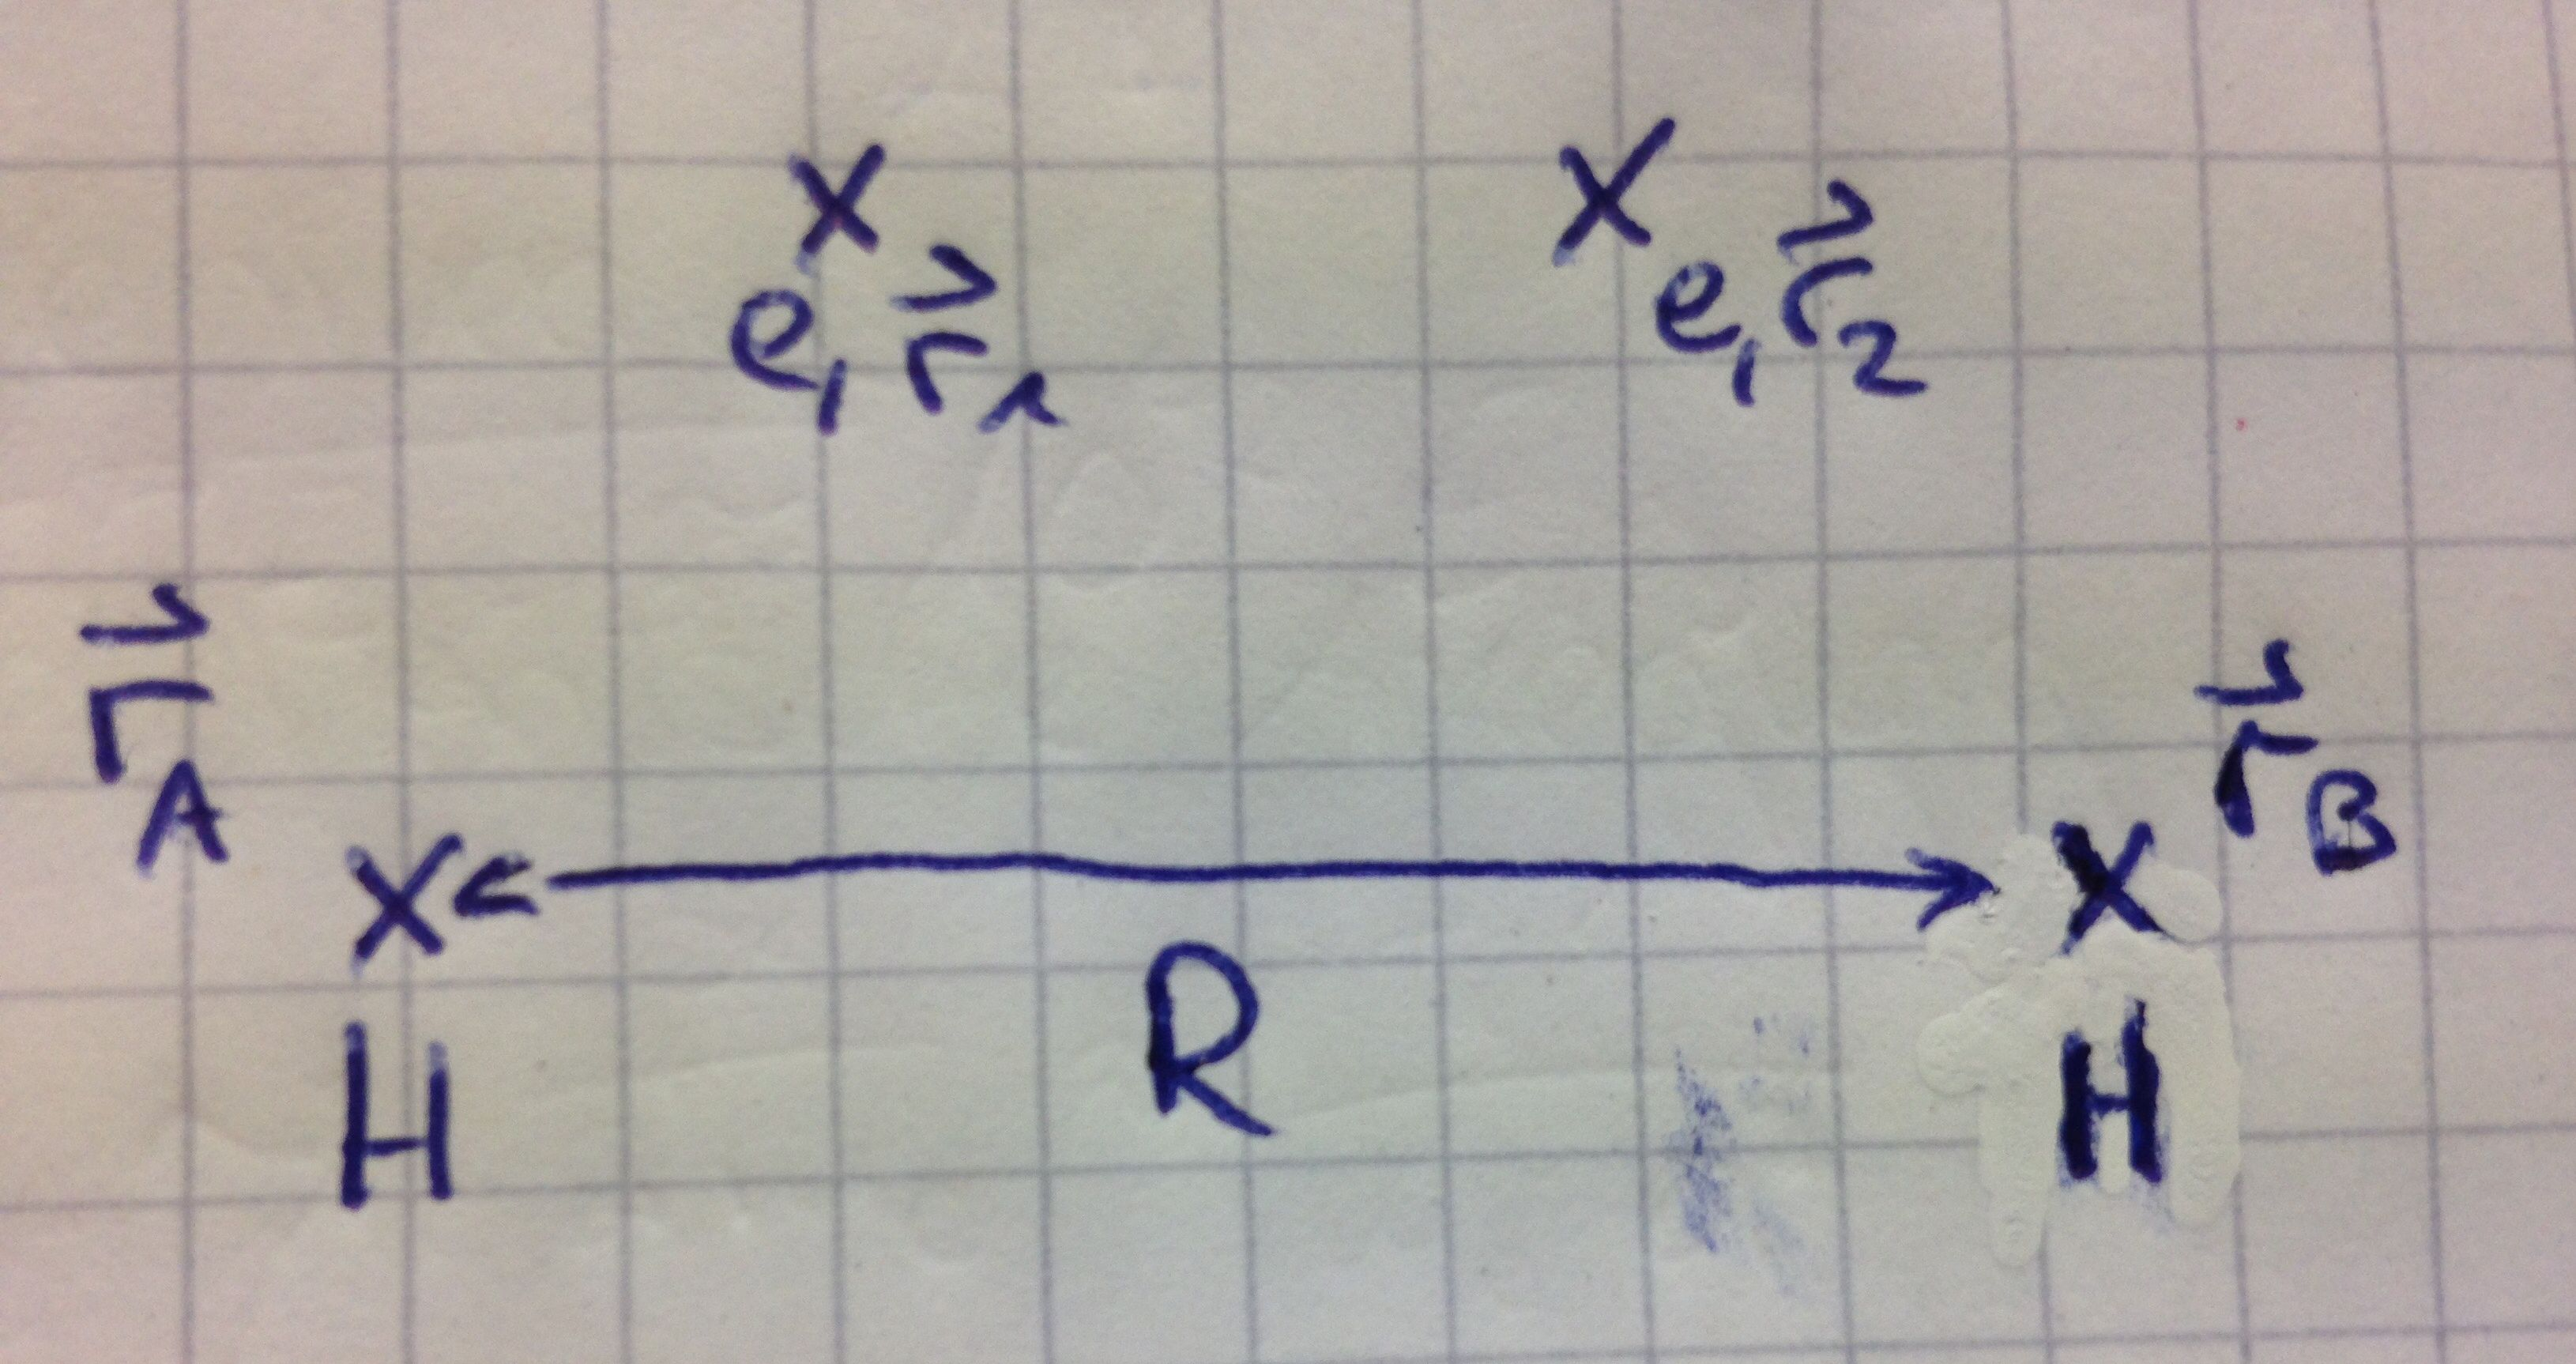
\includegraphics[width=10cm]{Homonukleare_Molekuele1}
		\end{center}
	\end{figure*}
	\begin{align*}
		R = | \vec{r}_A - \vec{r}_B |
	\end{align*}
	\begin{align*}
		R \rightarrow \infty &: \text{Separiert in 2 ``isolierte'' }H \text{-Atome} \\
		R \rightarrow 0 &: He\text{-Wellenfunktion}
	\end{align*}
Rotationssymmetrie gebrochen zu zylindrischer Symmetrie
	\begin{align*}
		C_\infty &\subset \mathscr{O} (3) 
		&\text{Homonuklear } C_{\infty_h} &= C_{\infty_h} \times C_i
	\end{align*}
$C_i$ ist die Parität

$L, J,$etc. keine ``guten'' Quantenzahlen.

Projektionvon $\vec{L}$ auf Molekühlachse $\Lambda$ ist erhalten
	\begin{align*}
		\Lambda &= 0, 1, 2, \ldots ,&
		\Lambda_z &= \pm \Lambda ~(\text{analog zu } m, \text{ aber } m = -\ell, +\ell) \\
		&\left(\Sigma, \Pi, \Delta, \text{etc.}\right)
		& ^{2S + 1}\Lambda &, \text{z.B. } ^3 \Pi ~(\text{Spin-Triplet}) 
	\end{align*}
Weitere Symmetrie: Spiegelung an Ebene
	\begin{figure*} [h]
		\begin{center}
			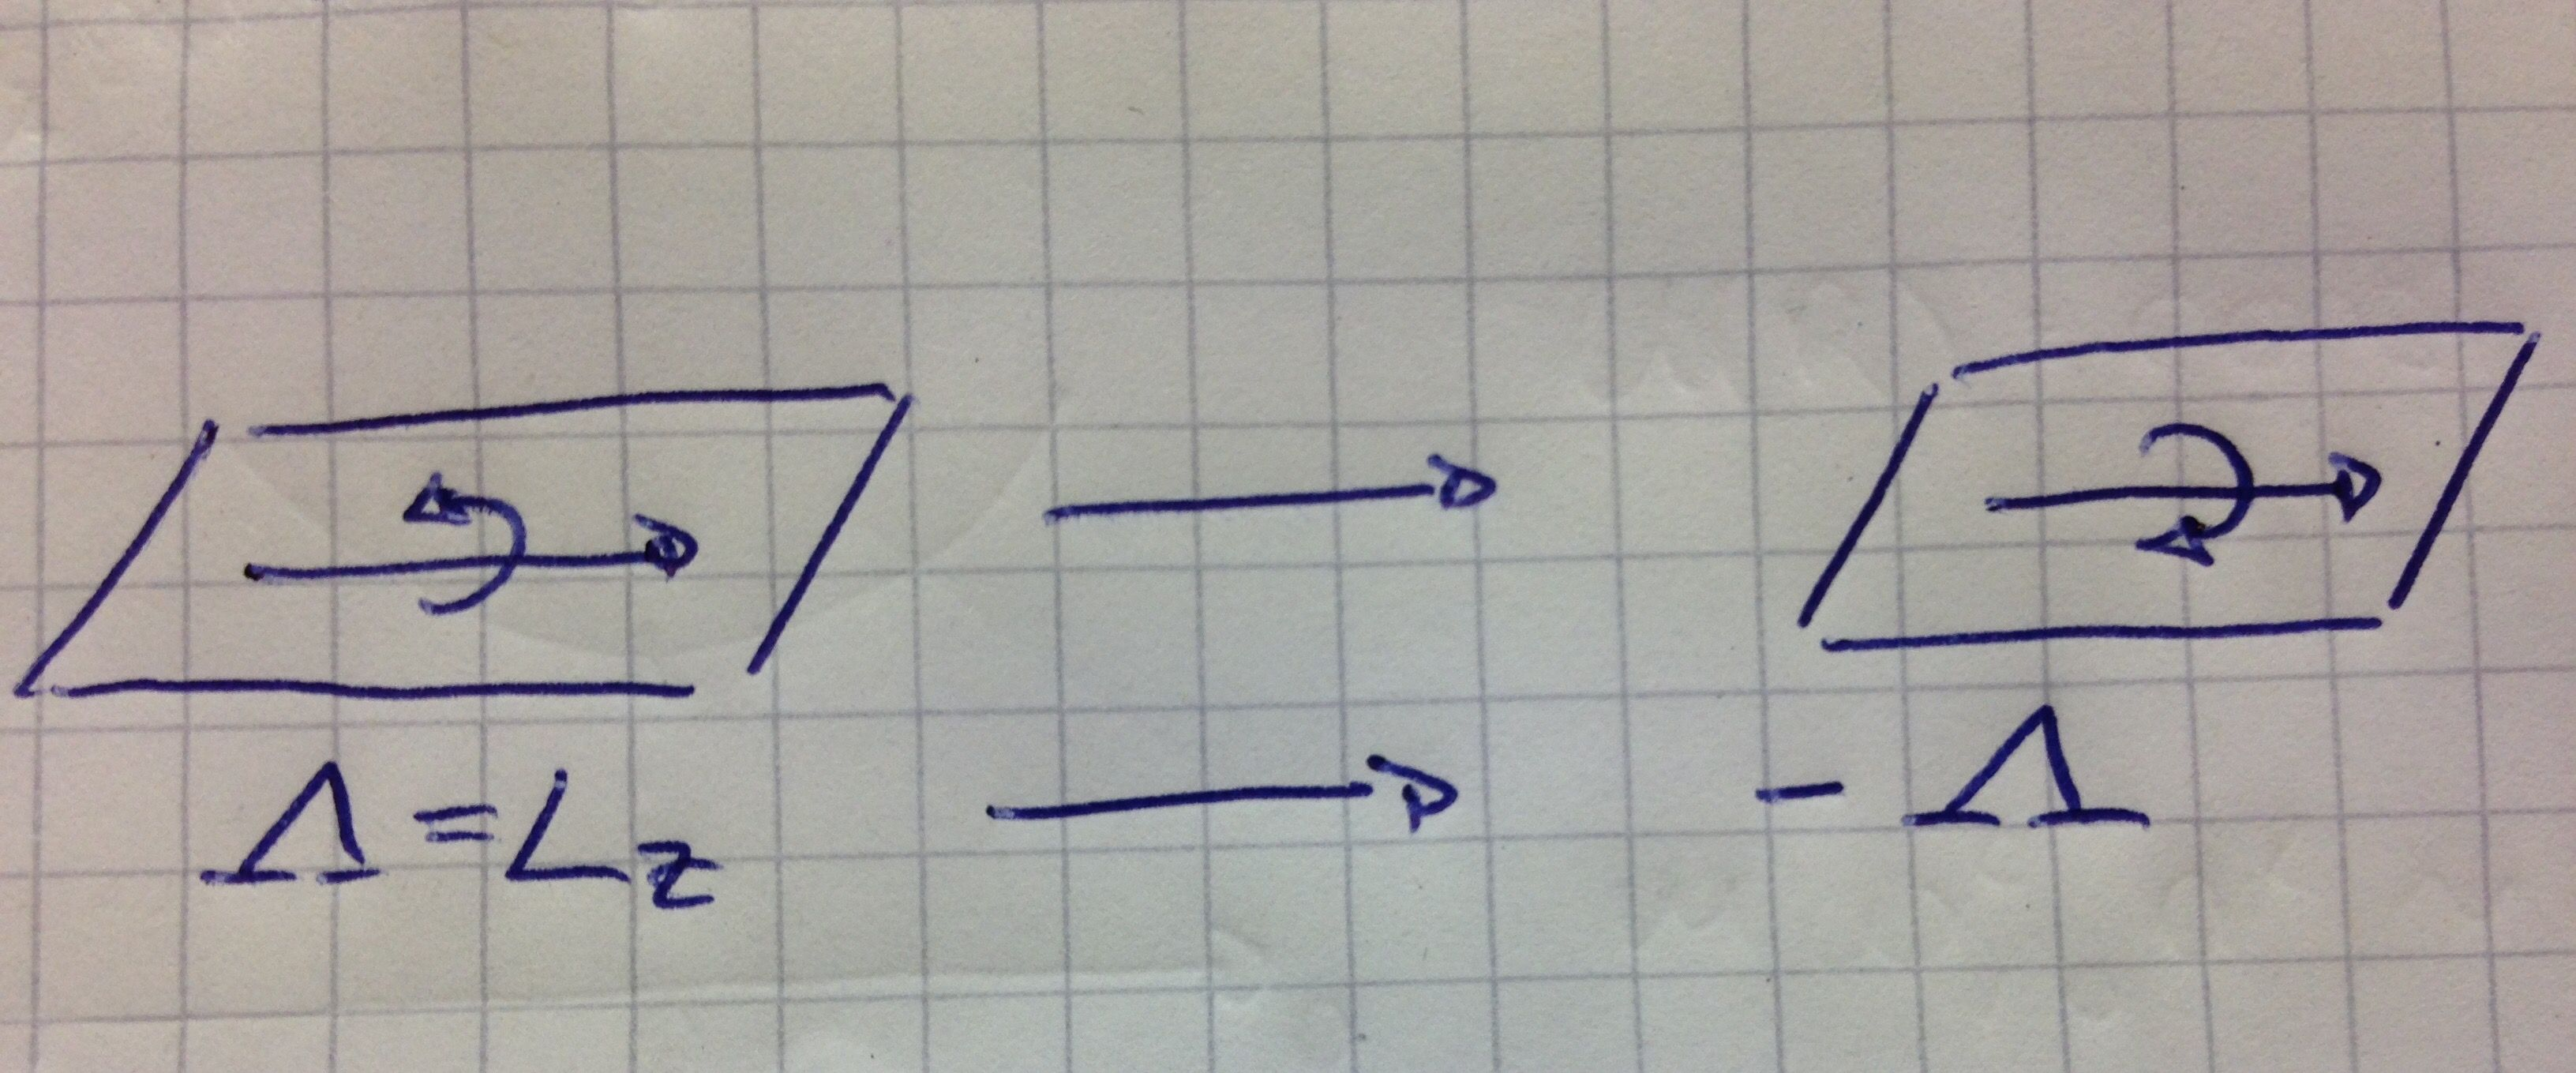
\includegraphics[width=10cm]{Homonukleare_Molekuele2}
		\end{center}
	\end{figure*}
	\begin{align*}
		\Lambda > 0 &: \text{Zustände sind 2-fach entartet. } (\text{analog zu } 2 \ell + 1 \text{ bei Rotationssymmetrie}) \\
		\Lambda = 0 &: \text{Eigenwerte } \sigma_V = + 1, \text{ oder } \sigma_V = -1.\\
		&\curvearrowright \Sigma^+ oder \Sigma^-
	\end{align*}
Homonuklear: Inversion am Mittelpunkt
	
$\Rightarrow$ Parität $\eta = g, u$ 
\\
Molekühlorbits:
	\begin{align*}
		^{2 S + 1}\Sigma_{g, u}^{+ , -} , ^{2 S + 1} \Pi_{g, u}, ^{2 S + 1}\Delta_{g, u}, \ldots
	\end{align*}
Grundzustand: Bahnwellenfunktion 

hat keine Knotetn $\curvearrowright \eta = g, \sigma_V = +$.
\\
Bahnwellenfunktion ist symmetrisch unter
	\begin{align*}
		\vec{r} \rightarrow - \vec{r} &\Rightarrow \text{ Spinwellenfunktion ist antisymmetrisch}\\
		&\Rightarrow S = 0
	\end{align*}
Wir interessieren uns für 	
	\begin{align*}
		^1\Sigma^+, ^1\Sigma^+_g ~(\text{homonuklear})
	\end{align*}
``Ausnahme'':
	\begin{align*}
		O_2 &: ^3\Sigma^-_g & &\text{hier kommen zeichnungen hin, }\\
		NO &: ^2\Pi & &\text{hab aber zu wenig ahnung von Chemielatexzeugsi}
	\end{align*}
	\begin{align*}
		R &\rightarrow 0 : He &\text{Parität } P &\rightarrow \eta = (-)^{S + L}
		&(\vec{r}_i \rightarrow -\vec{r}_i \text{ nicht } \vec{r}_1 \leftrightarrow \vec{r}_2) \\
		\Lambda &= 0 &\Sigma^{(-)^L \cdot \eta} &= \Sigma^{(-)^S}
	\end{align*}
$R \rightarrow 0$ verschiedene $D_{\infty_h}$ Zuständie geben dasselbe $J^{PC}$ (was das auch immer sein möge, ich hab echt keine Ahnung)

	\begin{tabular}{l l}
		He & H$_2$ \\
		$^1S_0$ & $^1\Sigma^+_g$ \\
		$^3S_1$ & $^3\Sigma^-_u$ \\
		$^1P_1$ & $^1\Sigma^+_u, ^1\Pi_u$\\
		$^3P_{0,1,2}$ & $^3\Sigma^-_g, ^3\Pi_g$\\
	\end{tabular}
	
Und hier war noch eine skurile Zeichnung, die keiner verstanden hat ;-)\\

$R \rightarrow \infty$ (2 isolierte $H$-Atome)\marginpar{26.11.15}
	\begin{align*}
		\left.
		\begin{aligned}
			2 \text{ mal } ^2S_{\frac{1}{2}} &\longrightarrow &
			S &= 0 & (\eta &= g) \\
			& & S &= 1 & (\eta &= \mu) 
		\end{aligned}
		\right\}
		\Lambda &= 0 ,~ \sigma_v  = +1
	\end{align*}
Grundzustand für $R \rightarrow \infty$ 
	\begin{align*}
		^1\Sigma^+_g &\text{ oder } ^3\Sigma^+_u
	\end{align*}
	\begin{figure*} [h]
		\begin{center}
			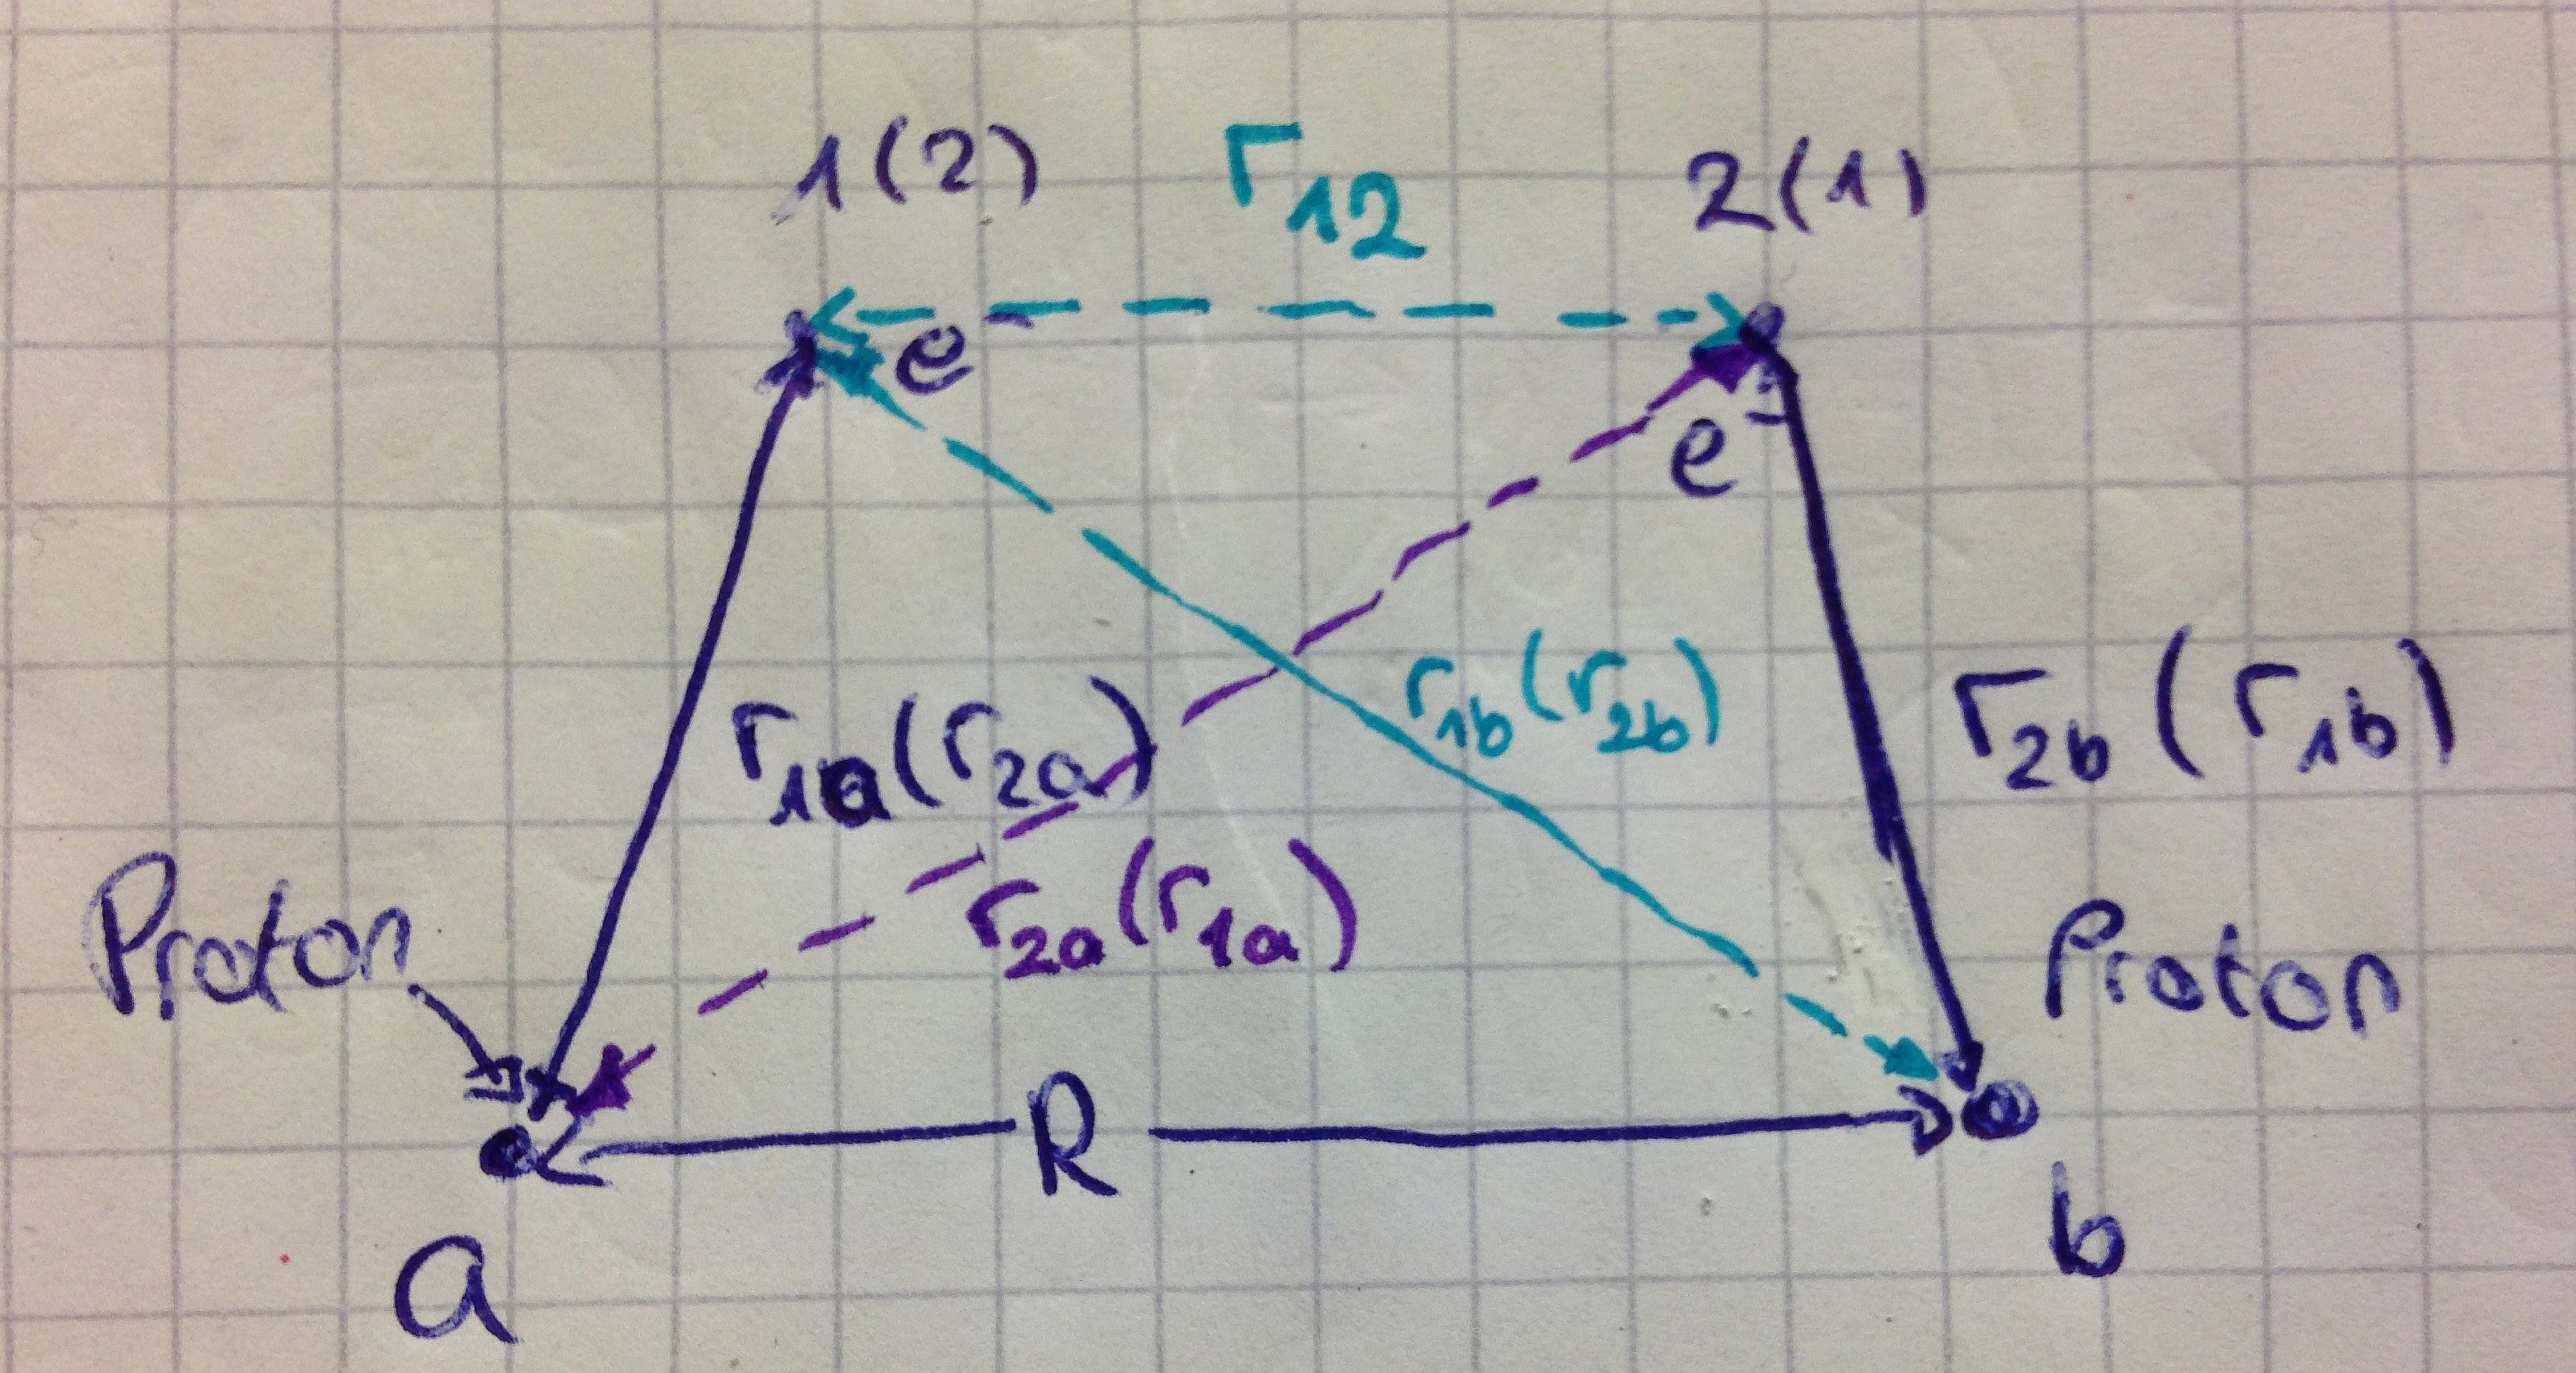
\includegraphics[width=10cm]{Homonukleare_Molekuele3}
		\end{center}
	\end{figure*}
	\begin{align*}
		\left(
		-\frac{\hbar^2}{2m_e} 
		\left(
		- \vec{\Delta}^2_1 - \vec{\Delta}^2_2
		\right) 
		V^{(R)}(\vec{r}_1, \vec{r}_2)
		\right)
		\Phi_n^{(R)} (\vec{r}_1, \vec{r}_2) 
		&= \U_n (R) \Phi_n^{(R)} (\vec{r}_1, \vec{r}_2) \\
		V^{(R)} (\vec{r}_1, \vec{r}_2) 
		&= \alpha \hbar c
		\left[
		\frac{1}{R} + \frac{1}{r_{12}} - \frac{1}{r_{1a}} - \frac{1}{r_{2b}} - \frac{1}{r_{1b}}
		- \frac{1}{r_{2a}}
		\right] \\
		(r_{12}, r_{1b} \text{ etc. Funktion von } R,\vec{r}_1, \vec{r}_2)
	\end{align*}
Betrachte Bahnwellenfunktion für große R:

Wasserstoffgrundzustand:
	\begin{align*}
		\psi (\vec{r}) &= \frac{1}{\sqrt{\pi a_{\mathrm{B}}^3}}
		e^{-\frac{r}{a_{\mathrm{B}}}} ,&
		E_1 &= -\frac{\alpha \hbar c}{2 a_{\mathrm{B}}} ,&
		a_{\mathrm{B}} &= \frac{\hbar}{m c \alpha} \text{ Bohr-Radius}
	\end{align*}
Ansatz für Wellenfunktion $\Phi(\vec{r}_1, \vec{r}_2)$
	\begin{align*}
		\Phi_1 (\vec{r}_1, \vec{r}_2) &= \psi (r_{1a}) \psi(r_{2b}) \\
		\Phi_2 (\vec{r}_1, \vec{r}_2) &= \psi (r_{1b}) \psi(r_{2a})
	\end{align*}
Heitler-London (1927) Ansatz:
	\begin{align*}
		\Phi^g &\propto \Phi_1 + \Phi_2 ,&
		\Phi^u &\propto \Phi_1 - \Phi_2
	\end{align*} 
Testwellenfunktion für Variationsverfahren
	\begin{align*}
		\ket{\Phi} &= \ket{\Phi_1} + \lambda \ket{\Phi_2}
		& \lambda \in \mathds{R} \text{ ist freier Parameter}
	\end{align*}
	\begin{align*}
		\U_0 \leq W(R) &=
		\frac{\braket{\Phi_1 + \lambda \Phi_2 | H | \Phi_1 + \lambda \Phi_2}}{\braket{\Phi_1 + \lambda \Phi_2 | \Phi_1 + \lambda \Phi_2}} \\
		&= \frac{\braket{\Phi_1 | H | \Phi_1} + \lambda^2 \braket{\Phi_2 | H | \Phi_2} + 2 \lambda \mathrm{Re} \left(\braket{\Phi_1 | H | \Phi_2}\right)}{1 + \lambda^2 + 2 \lambda \mathrm{Re} \braket{\Phi_1 | \Phi_2}} \\
		&= \frac{(1 + \lambda^2) H_{11} + 2 \lambda H_{12}}{1 + \lambda^2 + 2 \lambda S^2}
		(*)
	\end{align*} 
mit
	\begin{align*}
		H_{11} &= \braket{\Phi_1 | H | \Phi_1} = \braket{\Phi_2 | H | \Phi_2}\\
		H_{12} &= \mathrm{Re} \braket{\Phi_1 | H | \Phi_2}\\
		S^2 &= \mathrm{Re} \braket{\Phi_1 | \Phi_2} \rightarrow
		\left\{
		\begin{aligned}
			1 &,~ R \rightarrow 0 \\
			0 &,~ R \rightarrow \infty
		\end{aligned}
		\right.
	\end{align*}
Wie muss ich $\lambda$ wählen, damit $W(R)$ minimal ist?
	\begin{align*}
		\frac{\partial W}{\partial \lambda} 
		&= \frac{(2 \lambda H_{11} + 2 H_{12}) (1 + \lambda^2 + 2 \lambda S^2) - (2 \lambda + 2 S^2) ((\lambda^2 + 1)H_{11} + 2 \lambda H_{12})}{(\lambda^2 + 2 \lambda S^2 + 1)^2}
		= 0 \\
		\frac{\partial W}{\partial \lambda} &\propto \ldots 
		= (H_{12} - H_{11} S^2) (1 - \lambda^2)\\
		&\Rightarrow \lambda = + 1 \text{ oder } \lambda = -1
	\end{align*}
(Heitler - London Ansatz ergibt sich als Lösung des Variationsproblems)
	\begin{align*}
		\lambda &= \pm 1 \Rightarrow \U^{g \text{ oder }u} (R) 
		\overset{*}{\leq} \frac{H_{11} \pm H_{12}}{1 \pm S^2} \\
		S^2 &= \mathrm{Re}\braket{\Phi_1 | \Phi_2} 
		= \mathrm{Re} \int \diff^3 r_1 \diff^2 r_2 \psi^* (r_{1a}) \psi^* (r_{2b}) \psi(r_{1b}) \psi (r_{2a}) \\
		&= \mathrm{Re} \left(\int \diff^3 r_1 \psi^*(r_1a) \psi (r_{1b})\right)^2 \\
	\end{align*}
	\begin{align*}
		H_{11} &= \braket{\Phi_1 | H | \Phi_2} =
		\frac{\alpha \hbar c}{R} + 2 E_1 + K(R)
	\end{align*}
Wobei 
	\begin{align*}
		K(R) &= \alpha \hbar c \int \diff^3 r_1 \diff^3 r_2 |\psi (r_1a)|^2 
		|\psi (r_{2b})|^2 \left(\frac{1}{r_{12}} - \frac{1}{r_{2a}} - \frac{1}{r_{1b}}\right) \\
		&= \text{ Coulombpotential}
	\end{align*}
	\begin{align*}
		H_{12} = \mathrm{Re} (\braket{\Phi_1 | H | \Phi_2}) 
		= \left(\frac{\alpha \hbar c}{R} + 2 E_1\right) S^2 + A(R) 
	\end{align*}
mit 
	\begin{align*}
		A(R) &= \alpha \hbar c \mathrm{Re} \int \diff^3 r_1 \diff^3 r_2 \psi^* (r_{1a}) \psi^* (r_{2b}) \psi(r_{1b}) \psi (r_{2a}) \left(\frac{1}{r_{1a}} - \frac{1}{r_{2a}} - \frac{1}{r_{1b}}\right)\\
		&= \text{ Austauschintegral}
	\end{align*}
	\begin{align*}
		\U^{g \text{ oder }u} (R) &\leq 2 E_1 + \frac{\alpha \hbar c}{R} + 
		\frac{K(R) \pm A(R)}{1 \pm S^2(R)} \\
		R \text{ klein}:& \\
		S^2 &= 1 + \mathscr{O} (R^2) ,&
		K(R) &= - \frac{11}{8} \frac{\alpha \hbar c}{a_{\mathrm{B}}} + \mathscr{O} (R) \\
		& & &= A(R) + \mathscr{O} (R)\\
		&\overset{R \text{ klein}}{\Rightarrow} U^g - 2E_1 = \alpha \hbar c 
		\left(\frac{1}{R} - \frac{11}{8 a_{\mathrm{B}}}\right) 
	\end{align*}
	\begin{figure*} [h]
		\begin{center}
			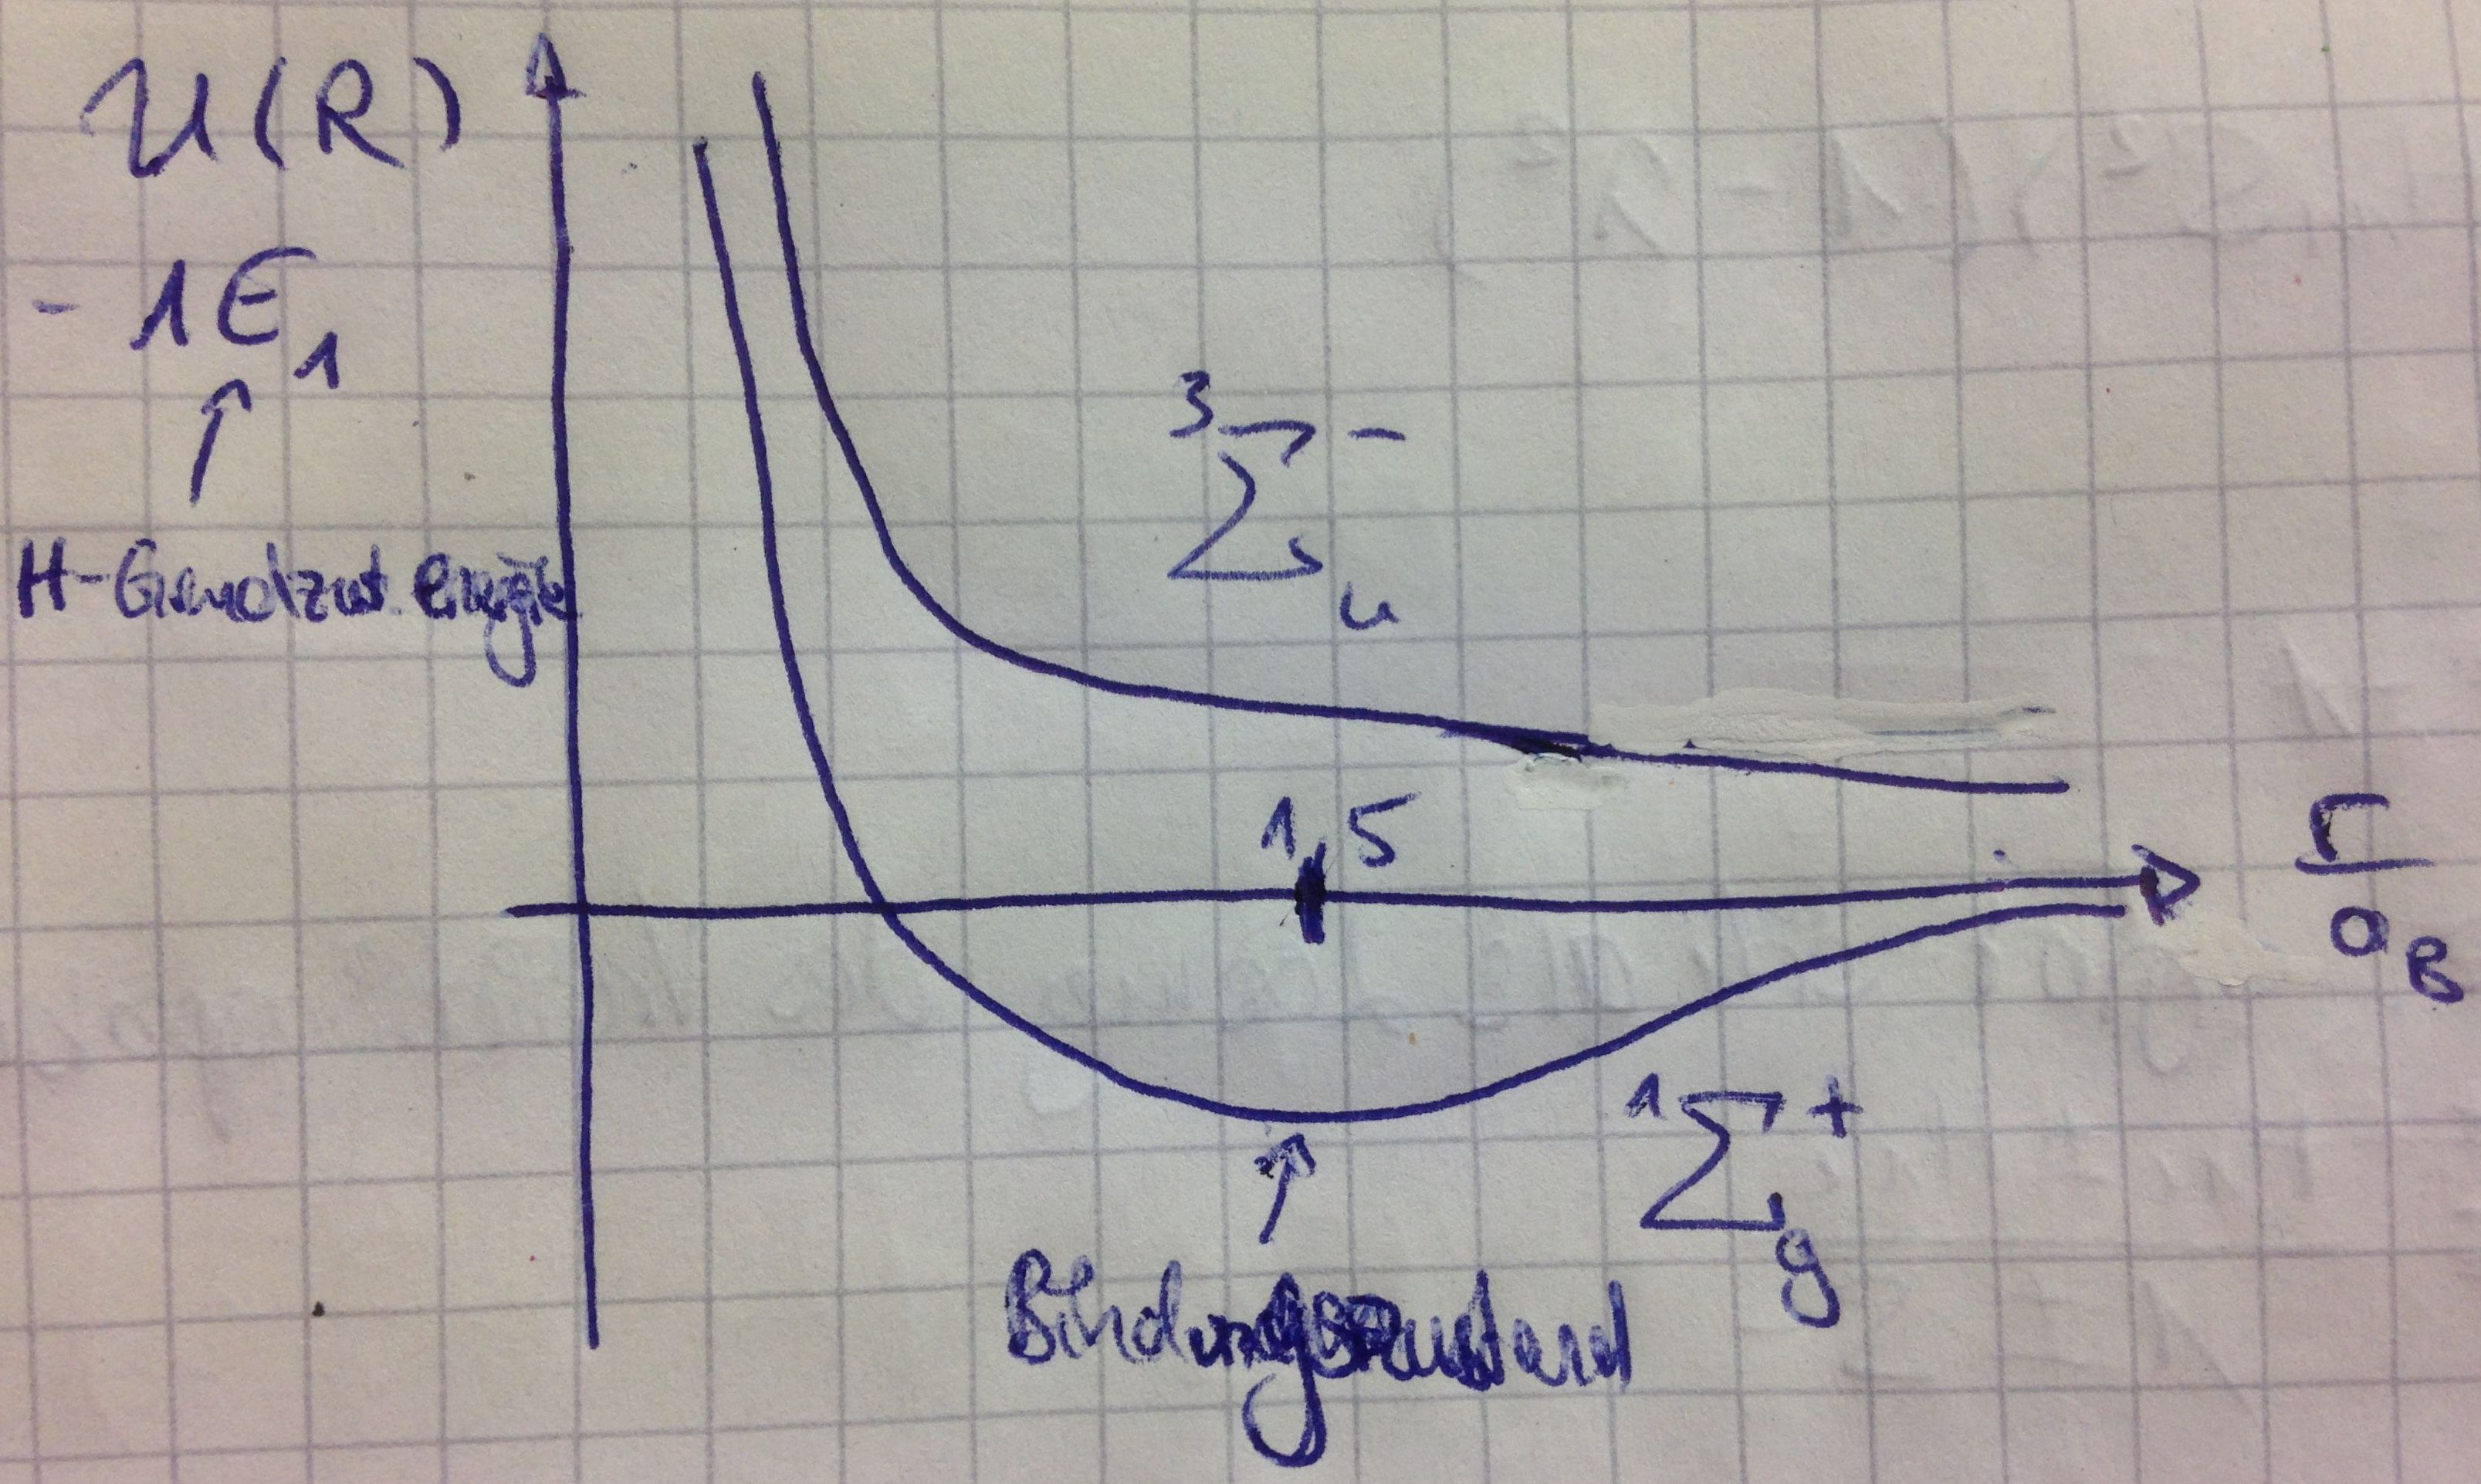
\includegraphics[width=10cm]{Homonukleare_Molekuele4}
		\end{center}
	\end{figure*}
\FloatBarrier
	\begin{tabular}{l | c | c | c}
		 & Heitler-London & Variation mit $Z \rightarrow Z^+ \mp 1$ & Natur \\
		 \hline 
		Bandlänge: $R_0$ & 0,08 nm & 0,076 nm & 0,074 nm \\
		Bindungsenergie: $\U (R_0) - 2E_1$ & $-3,14 e$V & $-3,76 e$V & $-4,48 e$V \\ 
	\end{tabular}
